%% Based on a TeXnicCenter-Template by Gyorgy SZEIDL.
%%%%%%%%%%%%%%%%%%%%%%%%%%%%%%%%%%%%%%%%%%%%%%%%%%%%%%%%%%%%%

%----------------------------------------------------------
%
\documentclass{article}%
%
%----------------------------------------------------------
% This is a sample document for the standard LaTeX Book Class
% Class options
%       --  Body text point size:
%                        10pt (default), 11pt, 12pt
%       --  Paper size:  letterpaper (8.5x11 inch, default)
%                        a4paper, a5paper, b5paper,
%                        legalpaper, executivepaper
%       --  Orientation (portrait is the default):
%                        landscape
%       --  Printside:   oneside, twoside (default)
%       --  Quality:     final(default), draft
%       --  Title page:  titlepage, notitlepage
%       --  Columns:     onecolumn (default), twocolumn
%       --  Start chapter on left:
%                        openright(no, default), openany
%       --  Equation numbering (equation numbers on right is the default):
%                        leqno
%       --  Displayed equations (centered is the default):
%                        fleqn (flush left)
%       --  Open bibliography style (closed bibliography is the default):
%                        openbib
% For instance the command
%          \documentclass[a4paper,12pt,reqno]{book}
% ensures that the paper size is a4, fonts are typeset at the size 12p
% and the equation numbers are on the right side.
%

% We use a lot of verbatim text. To get a better readability it's required to enlarge the line spacing.
\linespread{1.02}

\usepackage{amsmath}%
\usepackage{amsfonts}%
\usepackage{amssymb}%
\usepackage{graphicx}

% For rotating figures, tables, etc. including their captions
\usepackage{rotating}

%\usepackage{pdflscape}

\usepackage{wrapfig}
%\usepackage{subcaption}

\usepackage{scrextend}

% Using the export key with adjustbox, this will load the graphicx package, 
% and allow you to use its keys as part of \includegraphics.

\usepackage[export]{adjustbox}% http://ctan.org/pkg/adjustbox

% for arrows
\usepackage{tikz}
\usetikzlibrary{arrows.meta}

% For customization og description list
\usepackage{enumitem}

% for secttion related numbering of the figures
\usepackage{chngcntr}
\counterwithin{figure}{section}

%\usepackage{hyperref}
%\hypersetup{
%    colorlinks=true,
%    linkcolor=cyan,
%    filecolor=magenta,      
%    urlcolor=blue,
%    pdftitle={Overleaf Example},
%    pdfpagemode=FullScreen,
%    }

%\urlstyle{same}

\usepackage{xr}
\usepackage{nameref}
\usepackage{caption}

%----------------------------------------------------------
\newtheorem{theorem}{Theorem}
\newtheorem{acknowledgement}[theorem]{Acknowledgement}
\newtheorem{algorithm}[theorem]{Algorithm}
\newtheorem{axiom}[theorem]{Axiom}
\newtheorem{case}[theorem]{Case}
\newtheorem{claim}[theorem]{Claim}
\newtheorem{conclusion}[theorem]{Conclusion}
\newtheorem{condition}[theorem]{Condition}
\newtheorem{conjecture}[theorem]{Conjecture}
\newtheorem{corollary}[theorem]{Corollary}
\newtheorem{criterion}[theorem]{Criterion}
\newtheorem{definition}[theorem]{Definition}
\newtheorem{example}[theorem]{Example}
\newtheorem{exercise}[theorem]{Exercise}
\newtheorem{lemma}[theorem]{Lemma}
\newtheorem{notation}[theorem]{Notation}
\newtheorem{problem}[theorem]{Problem}
\newtheorem{proposition}[theorem]{Proposition}
\newtheorem{remark}[theorem]{Remark}
\newtheorem{solution}[theorem]{Solution}
\newtheorem{summary}[theorem]{Summary}
\newenvironment{proof}[1][Proof]{\textbf{#1.} }{\ \rule{0.5em}{0.5em}}

\setlength{\parindent}{0pt}

\newcommand{\must}{\textbf{must }}
\newcommand{\mustnot}{\textbf{must not }}
\newcommand{\required}{\textbf{required }}
\newcommand{\shall}{\textbf{shall }}
\newcommand{\shallnot}{\textbf{shall not }}
\newcommand{\should}{\textbf{should }}
\newcommand{\shouldnot}{\textbf{should not }}
\newcommand{\recommended}{\textbf{recommended }}
\newcommand{\may}{\textbf{may }}
\newcommand{\optional}{\textbf{optional }}

\newcommand{\private}{\indent\hspace{1.1cm} \textit{Don't use it for extensions.} \\ }
\newcommand{\public}{\indent\hspace{1.1cm} \textit{Can / must be used for extensions.} \\ }
\newcommand{\partially}{\indent\hspace{1.1cm} \textit{Some classes can / must be used for extensions.} \\ }


%%%%%%%%%%%%%%%%%%%%%%%%%%%%%%%%%%%%%%%%%%%%%%%%%%%%%%%%%%%%%

\begin{document}



\title{Fsk Encoder Developers Guide}
\author{\copyright \space The Fsk Encoder project}
\date{October 2025}
\maketitle


\tableofcontents
\listoffigures

\newpage

%%%%%%%%%%%%%%%%%%%%%%%%%%%%%%%%%%%%%%%%%%%%%%%%%%%%%%%%%%%%%

\textbf{Introduction}
\\

The Fsk Encoder application is a useful tool for SW development in retro computing environment.
\\
It's capable of converting binary code or data files into FSK encoded sound samples which can be played on the computers sound card. With an appropriate interconnection cable, the sound output of the host computer can be connected to the sound input of a retro computer system to upload code or data.
\\

Also it's extendible to support new target systems or different source file formats.
\\

This document gives (hopefully) all information needed to set up the Eclipse project for program maintenance and extension development.
\\

For a better understanding of this document, please refer to the Javadoc of the API classes and interfaces which can be found in the subpackages of the \verb|extension| package.


%%%%%%%%%%%%%%%%%%%%%%%%%%%%%%%%%%%%%%%%%%%%%%%%%%%%%%%%%%%%%

\newpage
\section{Project setup}
\label{Project-setup}
The project is split into two parts:

\begin{enumerate}

	\item The FskEncoder-Application, which is only a 'mainframe' and needs at least one input file reader and one target system extension to be ready for work. It can be downloaded from Github \\
	\verb|https://github.com/kamaso-macha/FskEncoder-Application|.
	
	\item The FskEncoder-Extension, which serves the different file reader and target system extensions. This project can also be downloaded from Github using the URL \\
	\verb|https://github.com/kamaso-macha/FskEncoder-Extensions|.

\end{enumerate}


%===============================================================================

\subsection{3pty Libraries}

External (3pty) libraries can be used but it's a good advice not to overdo it. This means, that if there is a low effort to write the code for a functionality, then do it instead of acquiring and installing an external library. 
\\

3pty libraries \should be imported by Maven. Only if there is no Maven repository for the required library, a manual download into the directory \verb|./lib| is permitted and the library must be manually added to the build path. However, this exception \must be documented in the extension's documentation.

%===============================================================================

\subsection{Default configuration}

The \verb|./cfg| directory contains a default Plugin.properties file which defines the built-in extension modules. It \must be left unchanged when building and distributing extensions. Instead, provide the extension configuration in a file named \verb|<extension_name>.properties|.
\\

It's also always welcome to add a readme file containing the code needed to patch the Fskencoder.bat file. That's in particular the extension of the class path for the extension itself and where applicable the class path of the used libraries.

%===============================================================================

\subsection{Building}

Apache ANT is used for building.
\\

For each extension, a buildfile \must be provided in the directory \verb|./build|. This buildfile is responsible for the build of only one specific extension and \should be named after the extension e.g.\\
\textit{BinReaderExtension.xml} for the BinReaderExtension.
\\

A second level buildfile \verb|BuildExtensions.xml| in the projects root directory builds \textbf{all} extensions by iterating over the files in the \verb|./build| directory.
\\

Commonly used properties and macros are put into the file \\
\verb|ExtensionsBuildSupport.xml|.



%%%%%%%%%%%%%%%%%%%%%%%%%%%%%%%%%%%%%%%%%%%%%%%%%%%%%%%%%%%%%

\section{Architectural overview}
\label{Architectural-overview}
%\externaldocument{ProjectSetup}

The FskEncoder follows the linear MVC model where only two interaction paths are possible:

\begin{enumerate}

	\item between View and Control and vice versa,
	
	\item between Control and Model and vice versa.
	
\end{enumerate}

\begin{figure}[h!]

	\includegraphics[width=\linewidth, keepaspectratio]{./images/ArchitectureOverview.png}
  \caption{Architecture overview}
  \label{fig:architecture-overview}
	
\end{figure}

\begin{minipage}{0.45\textwidth}

	The right-hand side shows the main window with two regions marked with a red frame.
	\\
	The top-one, with the caption \textit{Region}\, is the extension GUI of the input reader extension while the lower one (with the field \textit{File Name}\,) is from target system extension.
	\\
	
	These GUI parts are specific to each extension and are part of the extension packages.

\end{minipage}
\hfill % pushes the two pages to the margins, leaving a gap
\begin{minipage}{0.45\textwidth}

	% use adjustimage to get alignment option, 
	% \includegraphic would push the image out of the top of the page
	
	\adjustimage{width=\textwidth, valign=t}{./images/Mainwindow.png}
	\captionof{figure}{Main widow}
	
	% note that \textwidth will be the width of the minipage
\end{minipage}

\vspace{3 ex}

Figure \ref{fig:architecture-overview}\, \textit{\nameref{fig:architecture-overview}}\, depicts the global structure of the application together with the extensions:

\begin{itemize}

	\item \textbf{View} This is the main window with all GUI elements exept that of the GUI extensions.

	\item \textbf{Control} This is the control for the main window dealing with every thing exept the extension GUIs.

	\item \textbf{Workflow engine} Encapsulates the \textit{business logic}\, of the FskEncoder application and the extensions.

	\item \textbf{Model} The data model of the application. It holds some run-time data and the paroerties of the two configuration files \textit{FskEncoder.properties}\, and \textit{Plugin.properties}\,.

	\item \textbf{Soundplayer} Plays the sound samples on the selected output device with the desired volume.

	\item \textbf{InputReader Extension view} This is the GUI part of the selected input reader extension and \must provide all informations needed to deal with the input format.
	\\
	The example in the figure above shows the GUI of the Ihx8InputReaderExtension which can handle more than one memory section in a single file.

	\item \textbf{InputReader Extension control} Extension specific control which must handle all controls of the extension gui.

	\item \textbf{TargetSystem Extension view} This is the GUI part of the selected target system extension and \must provide all informations needed to deal with the specific protocol format.

	\item \textbf{TargetSystem Extension control} Extension specific control which must handle all controls of the extension gui.

	\item \textbf{TargetSystem Extension protocol} The protocol used to encode the binary data and to convert them into sound samples.

\end{itemize}

Each input reader and target system extension must be fully decoupled from the FskEncoder source (except the interface / base classes needed) and \shall only interact with the application via the provided interfaces.
\\

A deep dive into how to build those extensions is discussed in the section \ref{extension-instantiation}  \textit{\nameref{extension-instantiation}}\, on page \pageref{extension-instantiation}.
\\

By rule, the application itself and each extension lives in it's own .jar file which must contain all the necessary classes but no 3pty libraries (please refer to section \ref{Project-setup}   \textit{\nameref{Project-setup}}\, on page \pageref{Project-setup} for library management).

%===============================================================================

\subsection{Project structure}

This section gives an explanation of the different packages and their purposes. The classes are only discussed if there is a real need for the understanding of building extensions. Most of this information can be found in the JavaDoc of the project.
\\

For each package is specified if its classes and interfaces should not, can or must be used in extensions.
\\

\subsection{Application part}

The following source folder / packages and their contents currently exist:

\begin{samepage}
	\begin{addmargin}[1cm]{0cm}
		\begin{verbatim}

    .
    +---src (folder)
         +---application
         +---control
         |   +---gui
         |   +---validator
         +---extension
         |   +---control
         |   +---encoder
         |   +---factory
         |   +---model
         |   +---protocol
         |   +---sond
         |   +---source
         |   +---target
         |   +---view
         +---model
         +---protocol
         +---sound
         +---view
             +---gui
						
		\end{verbatim}
	\end{addmargin}
\end{samepage}


%===============================================================================

\subsection{Packages of the 'src' folder}

%*******************************************************************************

\subsubsection{application}

\private

Contains the application class together with classes to handle cli parameter, some 'hard coded' properties and for program exit.

%*******************************************************************************

\subsubsection{control}

\private

Contains the controller logic for work-flow and background task execution.


%*******************************************************************************

\subsubsection{control.gui}

\private

Held all controllers for the basic GUI panels.

%*******************************************************************************

\subsubsection{control.validator}

\private

Contains various validators for the GUI elements.

%*******************************************************************************

\subsubsection{extension}

\public

This package provides the logic needed for extending the application. A deeper discussion can be found in section \ref{api}  \nameref{api} \, on page \pageref{api}.
\\
The content of this package is packed in a seperate file \textit{FskEncoderExtension.jar} \, during build process and \must be used as library in the extension part.


%*******************************************************************************

\subsubsection{extension.control}

\public

Contains classes and interfaces needed for extension controllers.


%*******************************************************************************

\subsubsection{extension.encoder}

\public

This is more a library of basic functionallity and contains all (currently) necessary classes for sound sample generation.
\\

Protocol specific encoders \must be placed in the package of the target system extension protocol. 
\\

Please refer to the \textit{Mpf1BitEncoder}\, class in the \textit{Microprecessor 1}\, extension to learn how to use the basic methods to build a complex protocol.


%*******************************************************************************

\subsubsection{extension.factory}

\public

This package is the place for the base classes and interfaces needed to build a extension factory.


%*******************************************************************************

\subsubsection{extension.model}

\public

This package contains all classes and interfaces of the data model needed to implement a input reader extension.


%*******************************************************************************

\subsubsection{extension.protocol}

\public

This package contains all classes and interfaces needed to implement a target system extension protocol.


%*******************************************************************************

\subsubsection{extension.sound}

\partially

This package contains the definition of the audio format of the FskEncoder soundplayer and is required in an extension protocol.


%*******************************************************************************

\subsubsection{extension.source}

\public

This package contains all classes and interfaces needed to implement a input reader extension.


%*******************************************************************************

\subsubsection{extension.target}

\public

This package is currently empty.


%*******************************************************************************

\subsubsection{extension.view.gui}

\public

Holds all base classes for extension guis.


%*******************************************************************************

\subsubsection{model}

\private

This package contains all classes of the internal data model.


%*******************************************************************************

\subsubsection{protocol}

\public

This package is currently empty.


%*******************************************************************************

\subsubsection{sound}

\private

All stuff around the sound player.


%*******************************************************************************

\subsubsection{view}

Currently empty.


%*******************************************************************************

\subsubsection{view.gui}

\private

Contains all classes needed for the main window and the basic GUI panels.


%===============================================================================

\subsection{Extensions part}

In the extension part are all packages located, which are related to extensions. They \must be strictly kept apart of the application part!

The following source folder / packages and their contents currently exist:

\begin{samepage}
	\begin{addmargin}[1cm]{0cm}
		\begin{verbatim}

    .
    +---src (folder)
        +---source
        |   +---bin
        |   +---ihx
        |       +---x8
        +---target
            +---microprofessor1
            +---z80trainer
						
		\end{verbatim}
	\end{addmargin}
\end{samepage}


%===============================================================================

\subsubsection{source.bin}

\private

Contains all sources for the binary input file reader.


%*******************************************************************************

\subsubsection{source.ihx}

\partially

Contains all common used sources for the Intel-Hex input file reader.


%*******************************************************************************

\subsubsection{source.x8}

\private

Contains the 8-bit specific implementation of the Ihx-reader extension.


%*******************************************************************************

\subsubsection{target.microprofessor1}

\private

Contains the classes of the Microprofessor 1 extension.


%*******************************************************************************

\subsubsection{target.z80trainer}

\private

Contains the classes of the Z80 trainer extension.





%%%%%%%%%%%%%%%%%%%%%%%%%%%%%%%%%%%%%%%%%%%%%%%%%%%%%%%%%%%%%

\section{API}
\label{api}
A input reader extension is at least based on four classes:

\begin{enumerate}

	\item a ReaderExtension,
	\item a ReaderGui
	\item a ReaderControl and
	\item a Reader.

\end{enumerate}

By convention, this classes \should be named like 

\begin{enumerate}

	\item \verb|<extension_name>|ReaderExtension,
	\item \verb|<extension_name>|ReaderGui
	\item \verb|<extension_name>|ReaderControl and
	\item \verb|<extension_name>|Reader,

\end{enumerate}

with \verb|<extension_name>| as descriptive name which reflects the format of the input file like \textit{Bin}\, for binary files or \textit{Ihx8}\, for Intel-Hex format.
\\

A target system extension requires at least the four classes

\begin{enumerate}

	\item Extension,
	\item ExtensionGui
	\item ExtensionControl and
	\item Protocol.

\end{enumerate}

The naming conventions follow the rules of the input reader and \should be like

\begin{enumerate}

	\item \verb|<extension_name>|Extension,
	\item \verb|<extension_name>|ExtensionGui
	\item \verb|<extension_name>|ExtensionControl and
	\item \verb|<extension_name>|Protocol,

\end{enumerate}


To build a apropriate memeory model for an extension, a input file reader \should use the classes of the \verb|extension.model| and \verb|extension.source| packages.

%*******************************************************************************

\subsection{Functional interface}

The communication between the main application and an extension is and \must be kept restricted to predefined methods to keep the dependencies between the application and the extension as low as possible. The methods used are discussed later in the deeper explanation of the differen parts of the extensions.

\begin{sidewaysfigure}

		\includegraphics[width=\linewidth,height=\textheight,keepaspectratio]{images/seq.UserInteraction.png}

    \caption{Sequence diagram of user interaction}

    \label{fig:seq-UserInteraction}
		
\end{sidewaysfigure}


Figure \ref{fig:seq-UserInteraction}\, \textit{\nameref{fig:seq-UserInteraction}}\,on page \pageref{fig:seq-UserInteraction} depicts how the application and the different parts of an extension work together.


%*******************************************************************************

\subsection{Extension instantiation}
\label{extension-instantiation}

Extensions are created in extension factories which are part of the extension itself. Theese extension factories are instantiated by the PluginFactory and the extension factory is responsible for creating the required model, controller and protocol classes.

\begin{sidewaysfigure}

		\includegraphics[width=\linewidth,height=\textheight,keepaspectratio]{images/seq.LoadExtensions.png}

    \caption{Example Sequence diagram of extension load process}

    \label{fig:seq.LoadExtensions}
		
\end{sidewaysfigure}

Page \pageref{fig:seq.LoadExtensions} shows the sequence diagram of the creation of an InputReaderExtension and TargetsystemExtension.


%*******************************************************************************

\subsection{Target system extension}

A target system extension provides all logic and functionality needed to translate the (binary) source data from the source buffer into the sound samples which can be played on the sound card of the host computer.
\\

It consists at least of:

\begin{enumerate}

	\item A extension factory, which is the implementation of the interface\\
	\verb|TargetSystemExtensionFactory| and will be discussed in more detail in the section \textit{\nameref{TargetSystemExtension}}\, below.
	
	\item The extension GUI, which \must extend the abstract \verb|ExtensionGui| base class and \must be implemented using Java Swing. It's recommend to use the \textit{miglayout}\, layout manager as the main window does.
	
	\item The controller logic (MVC model), which is derived from the abstract \\
	\verb|TargetSystemExtensionControl|.
	
	\item The so called 'protocol', which is capable for the translation process. \\
	It is an extension of the abstract \verb|BackgroundTaskProtokol| base class and \should use the various encoder classes of the \verb|extension.encoder| package for encoding sound samples.

\end{enumerate}

\begin{sidewaysfigure}

		\includegraphics[width=\linewidth,height=\textheight,keepaspectratio]{images/cls.target.z80trainer.png}

    \caption{Example Z80TrainerExtension class diagram}

    \label{fig:cls-target-z80trainer}
		
\end{sidewaysfigure}

Page \pageref{fig:cls-target-z80trainer} shows the class diagram of the Z80-Trainer extension as an example of how an target system extension is to build.

%*******************************************************************************

\subsubsection{TargetSystemExtension}
\label{TargetSystemExtension}

This factory class is responsible for the creation of the extensions MVC pattern and \must implement the \verb|TargetSystemExtensionFactory| interface. It must create an instance of the ExtensionControl and a \\
\verb|TargetSystemExtensionDao| which is later on registered in the application.
\\

Because this class is registered in the \textit{Plugin.properties}\, it \should be named like

\begin{itemize}

	\item[] \verb|<system_name>Extension| what results in a .jar file named
	\item[] \verb|<system_name>Extension.jar|.

\end{itemize}

\verb|<system_name>| is a descriptive name like \textit{Z80Trainer}\,, \textit{Mpf1}\, or anything else.


%*******************************************************************************

\subsubsection{TargetSystemExtensionGui}

Some transmission protocols need additional information which can't be obtained from the input file. This is e.g. the \textit{Program Number}\, of the Z80-Trainer.
\\
The TargetSystemExtensionGui is the place where to put those input fields.
\\
As said before, it \must be derived from the abstract class \verb|ExtensionGui| and is instantiated later on in the assocciated controller class.


%*******************************************************************************

\subsubsection{TargetSystemExtensionControl}

The TargetSystemExtensionControl must extend the abstract class \\
\verb|TargetSystemExtensionControl|.
\\

It \should at least

\begin{enumerate}

	\item create an instance of the protocol implementaion,
	
	\item create an instance of the related GUI and pass a referenze to itself,
	
	\item initialize the GUI with appropriate default values,
	
	\item implement the methods of the base class (which are inherited from Java Swing ActionListener) and 
	
	\item provide the handle methods for the GUI elements by implementing required Java Swing interfaces (like FocusListener, ChangeListener, ...).

\end{enumerate}

%*******************************************************************************

\subsubsection{TargetSystemProtocol}

The TargetSystemProtocol is derived from the abstract base class \\
\verb|BackgroundTaskProtokol|  and \must implement the two methods \verb|compile(...)| and \verb|setFullProgress(int)(...)|. \\
It \may override the \verb|setStartAddress(...)|, \verb|setEndAddress(...)| or \\
\verb|setSize(...)| methods with its own behavior.

%===============================================================================

\subsection{Input reader}

A input reader provides all functionality needed to read a data file in a specific format and to convert the data read into plain binary bytes. It builds a data buffer which later on is handed over to the protocol part of the target system extension.
\\

It consists at least of:

\begin{enumerate}

	\item A extension factory which is in fact the implementation of the \\
	\verb|InputReaderExtensionFactory| interface.
	
	\item The Java Swing extension GUI which must extend the \\ 
	abstract \verb|MemoryMapGui| base class.

	\item The controller logic (MVC model) which is derived from the abstract \\
	\verb|ReaderExtensionControl| and must implement the two Java Swing interfaces \verb|ChangeListener| and \verb|FocusListener|.

	\item The so called 'reader', which is capable for the translation process. \\
	It is an extension of the abstract \verb|ReaderBase| base class.
	
	\item An extension of the abstract \verb|MemoryRegionBuilder| class which provides the interface to the protocol implementation.
	
	\item Optionally an extension of the abstract base class \verb|Record| if the input file format is record structured.
	
\end{enumerate}

\begin{sidewaysfigure}

		\includegraphics[width=\linewidth,height=\textheight,keepaspectratio]{./images/cls.ext.source.bin.png}

    \caption{Example BinReaderExtension class diagram}

    \label{fig:clsBinReaderExtension}
		
\end{sidewaysfigure}

Page \pageref{fig:clsBinReaderExtension} shows the class diagram of the binary input file reader extension as an example of how an input reader extension is to build .

%*******************************************************************************

\subsubsection{ReaderExtension}

The ReaderExtension class is a factory which creates 

\begin{itemize}

	\item a instance of the \verb|MemoryMap| class,
	\item a instance of the \verb|Reader| class,
	\item a instance of the \verb|ReaderControl| class and

	\item a instance of the \verb|InputReaderExtensionDao|, which held references to the previous three classes.

\end{itemize}

The \verb|InputReaderExtensionDao| is returned to the caller \verb|PluginFactory| and further to \verb|WorkflowEngine|.
\\

This class is registered in the Extension.properties and should be named according to the rules previously stated in section \ref{TargetSystemExtension}  \textit{\nameref{TargetSystemExtension}}\, on page \pageref{TargetSystemExtension}.


%*******************************************************************************

\subsubsection{MemoryMapGui}

This base class provides a filed which holds a list of \verb|MemoryBlockDescription| objects. Each object of this list describes a memory block of the source file with the three attributes \textit{START\_ADDRESS}\,, \textit{END\_ADDRESS}\, and \textit{SIZE}. These attributes are required to set up the reader extension GUI.


%*******************************************************************************

\subsubsection{ReaderExtensionControl}

The ReaderExtensionControl must extend the abstract class \\
\verb|ReaderExtensionControl|.
\\

It \should at least

\begin{enumerate}

	\item create an instance of the reader implementaion,
	
	\item create an instance of the related GUI and pass a referenze to itself,
	
	\item initialize the GUI with appropriate default values,
	
	\item implement the methods of the base class (some inherited from Java Swing ActionListener), 
	
	\item provide the handle methods for the GUI elements by implementing required Java Swing interfaces (like FocusListener, ChangeListener, ...) and
	
	\item hold an instance of the \verb|MemoryMap| object.

\end{enumerate}

%*******************************************************************************

\subsubsection{Reader}

The Reader implementation \must be derived from the abstract \verb|ReaderBase| class and \must implement the inherited methods. 
\\

It's responsible for reading and parsing the input file and storing the file content in a \verb|MemoryRegion| object via a \verb|MemoryRegionBuilder| instance.


%*******************************************************************************

\subsubsection{MemoryRegionBuilder}

This is the storage container for the data red by the reader implementation. It extends the abstract \verb|MemoryRegionBuilder| and implements it's abstract methods.


%*******************************************************************************

\subsubsection{MemoryRegion}

A MemoryRegion represents a bunch of binary data together with it's start address and it's size.


%*******************************************************************************

\subsubsection{MemoryMap}

The MemoryMap holds a map of \verb|MemoryRegion| objects. It is responsible for creation of \verb|MemoryBlockDescription| objects used by the GUI and for delivery a specific \verb|MemoryRegion| on request.


%*******************************************************************************

\subsubsection{Record}

The input reader philosophy is based on the \textit{Record}\, structure because every input file can be transformed into records. A binary file contains only one record where on the other hand a Intel-Hex formatted file is strictly based on the record structure. To simplify the reading / parsing process and the  data handling, it is strongly adviced to rely on this philosophy.




%%%%%%%%%%%%%%%%%%%%%%%%%%%%%%%%%%%%%%%%%%%%%%%%%%%%%%%%%%%%%

\newpage
\appendix

\section{Nomenclature}
\label{Nomenclature}
\subsection{Keywords}

The key words \footnote{Taken from IETF RFC 2119, Key words for use in RFCs to Indicate Requirement Levels}
"MUST", "MUST NOT", "REQUIRED", "SHALL", "SHALL NOT", "SHOULD", "SHOULD NOT", "RECOMMENDED", "MAY", and
"OPTIONAL" in this document are to be interpreted as:

\begin{enumerate}

	\item MUST This word, or the terms "REQUIRED" or "SHALL", mean that the
definition is an absolute requirement of the specification.

	\item  MUST NOT This phrase, or the phrase "SHALL NOT", mean that the
definition is an absolute prohibition of the specification.

	\item  SHOULD This word, or the adjective "RECOMMENDED", mean that there
may exist valid reasons in particular circumstances to ignore a
particular item, but the full implications must be understood and
carefully weighed before choosing a different course.

	\item  SHOULD NOT This phrase, or the phrase "NOT RECOMMENDED" mean that
there may exist valid reasons in particular circumstances when the
particular behavior is acceptable or even useful, but the full
implications should be understood and the case carefully weighed
before implementing any behavior described with this label.

	\item MAY This word, or the adjective "OPTIONAL", mean that an item is
truly optional. One vendor may choose to include the item because a
particular marketplace requires it or because the vendor feels that
it enhances the product while another vendor may omit the same item.
An implementation which does not include a particular option MUST be
prepared to inter-operate with another implementation which does
include the option, though perhaps with reduced functionality. In the
same vein an implementation which does include a particular option
MUST be prepared to inter-operate with another implementation which
does not include the option (except, of course, for the feature the
option provides.)

\end{enumerate}


%===============================================================================

\subsection{UML grapics}

This document contains some UML class diagrams. In this diagrams are two styles used to draw the classes: 

\begin{itemize}

	\item	First the standard style, white background with attributes and methods defined for all classes / interfaces in the package of interest and
	
	\item second the greyed style, grey background and dashed lines, without definition of attributes and methods for all collabrating classes / interfaces of different packages.
	
\end{itemize}

The greyed classes / interfaces are included for completeness and to lay out the dependencies between packages.
\\

Arrows in the relationship of classes and interfaces and their meanign :
\\

\begin{addmargin}[1cm]{0cm}
	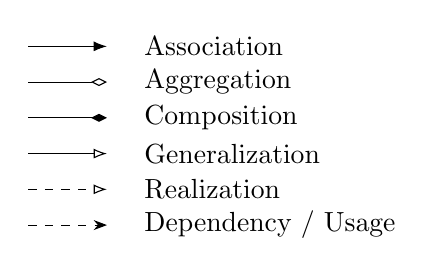
\begin{tikzpicture}[yscale=-1, y=3ex]

		\draw [-{Latex}]							(0, 1) to ++(1, 0) node [right] {\quad Association};
		\draw [-{Diamond[open]}]			(0, 2) to ++(1, 0) node [right] {\quad Aggregation};
		\draw [-{Diamond}]						(0, 3) to ++(1, 0) node [right] {\quad Composition};
		\draw [-{Latex[open]}]				(0, 4) to ++(1, 0) node [right] {\quad Generalization};
		\draw [-{Latex[open]},dashed]	(0, 5) to ++(1, 0) node [right] {\quad Realization};
		\draw [-{Stealth},dashed]			(0, 6) to ++(1, 0) node [right] {\quad Dependency / Usage};
		
	\end{tikzpicture}
\end{addmargin}

\vspace{2ex}

If two classes A and B have a relationship, than

\begin{description}[style=multiline,leftmargin=8em]
	
	\item[association] between A and B means that A hold a reference to B so that A can communicate with B,
	
	\item[aggregation] means, that A holds one or more refeerences to B,
	
	\item[composition] means, that B is part of A in that way, that B can't exist without A. 
	
	\item[generalization] is, when B extends A
	
	\item[realization] is, when A implements the interface B
	
	\item[dependency] means, that A uses B but without keeping a reference to B.

\end{description}




%===============================================================================

\end{document}
